\section{Struttura del database}

\subsection{Modello relazionale}
    \begin{figure}[h]
        \centering
        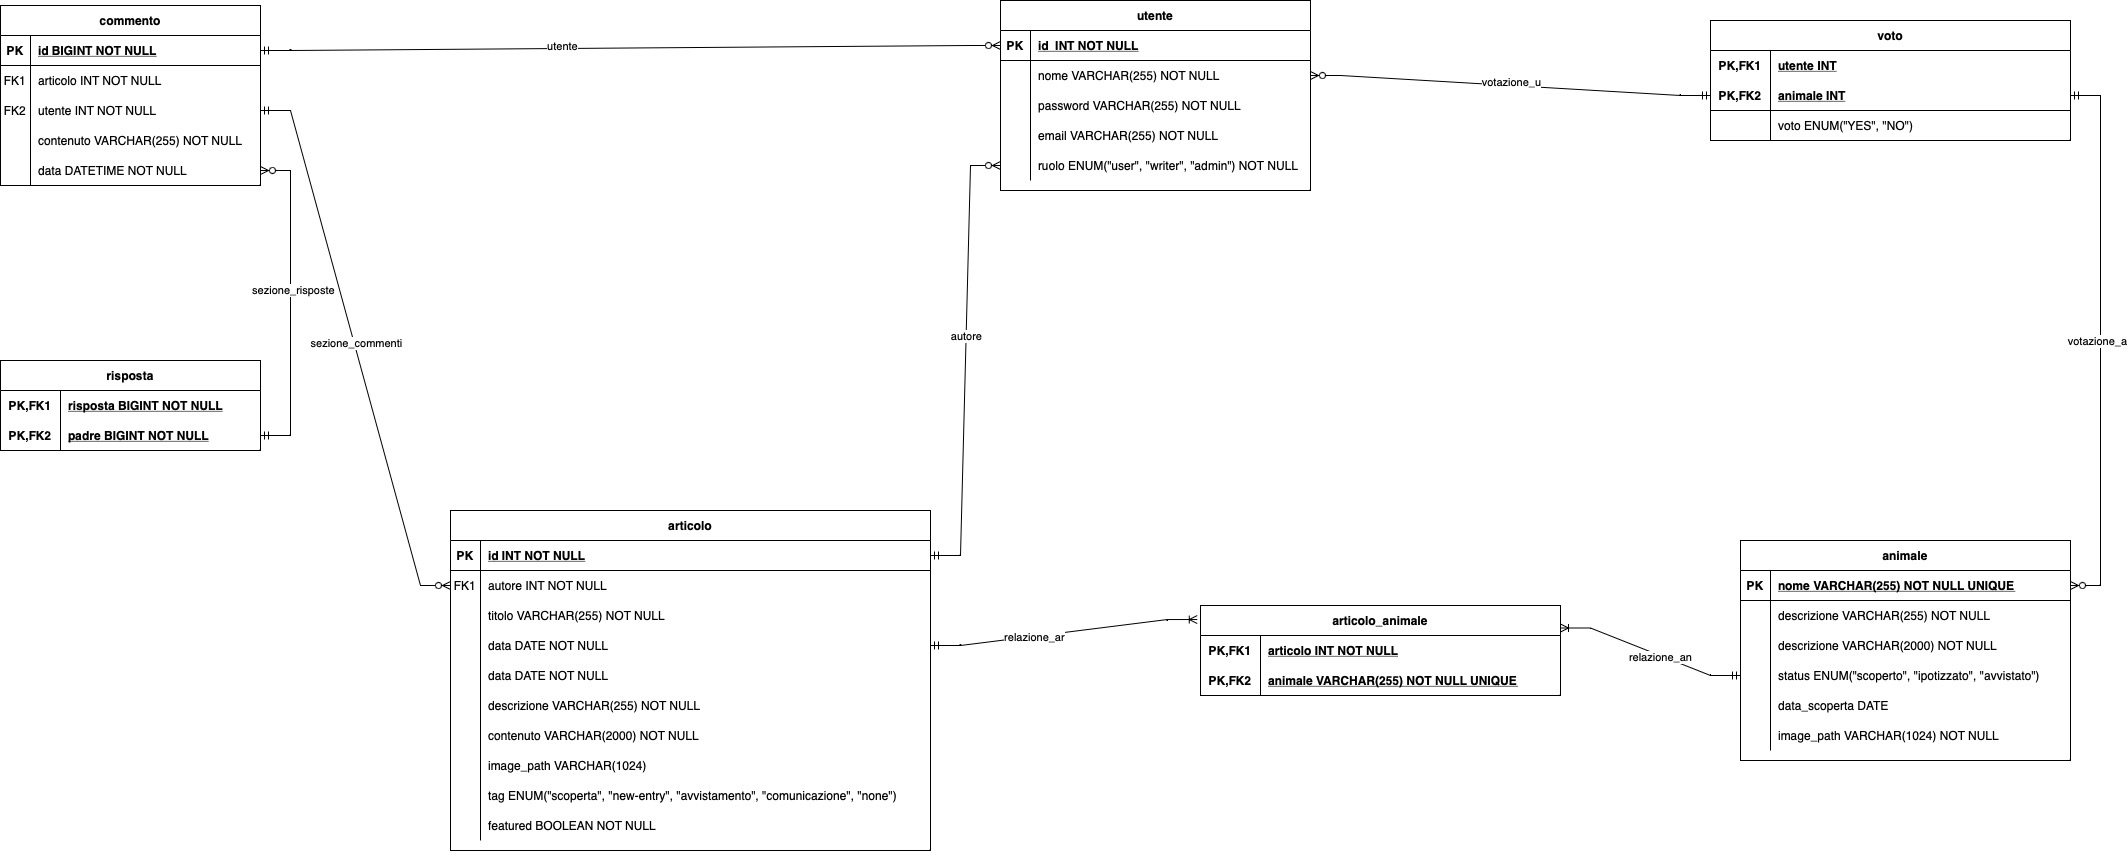
\includegraphics[width=1.0\textwidth]{assets/eLusive_DB.jpg}
        \caption{Diagramma ER}
        \label{fig:diagramma_er}
    \end{figure}

\subsection{Modello logico}
    \begin{itemize}
        \item \textbf{articolo}:
        \begin{itemize}
            \item \underline{id} 
            \item titolo
            \item autore (articolo.autore $\rightarrow$ utente.id)
            \item data
            \item descrizione
            \item contenuto
            \item immagine
            \item tag [\textbf{scoperta}, \textbf{new-entry}, \textbf{avvistamento}, \textbf{comunicazione}, \textbf{none}]
            \item featured
        \end{itemize}

        \item \textbf{articolo\_animale}:
        \begin{itemize}
            \item \underline{articolo} (articolo\_animale.articolo $\rightarrow$ articolo.id)
            \item \underline{animale} (articolo\_animale.animale $\rightarrow$ animale.nome)
        \end{itemize}

        \item \textbf{utente}:
        \begin{itemize}
            \item \underline{id}
            \item nome
            \item password
            \item email
            \item ruolo [\textbf{admin}, \textbf{writer}, \textbf{user}]
            \begin{itemize}
                \item \textbf{admin}: tutti privileggi [DA DEFINIRE NEL DETTAGLIO]
                \item \textbf{writer}: possono creare articoli, modificare e cancellare i propri articoli
                \item \textbf{user}: ovvero utenti registrati che possono leggere, commentare gli articoli e votare
            \end{itemize}
        \end{itemize}

        \item \textbf{commento}:
        \begin{itemize}
            \item \underline{id}
            \item articolo (commento.articolo $\rightarrow$ articolo.id)
            \item utente (commento.utente $\rightarrow$ utente.id)
            \item data
            \item contenuto
        \end{itemize}

        \item \textbf{risposta}
        \begin{itemize}
            \item \underline{risposta} (risposta.risposta $\rightarrow$ commento.id)
            \item \underline{padre} (risposta.padre $\rightarrow$ commento.id)
        \end{itemize}

        \item \textbf{voto}:
        \begin{itemize}
            \item \underline{utente} (voto.utente $\rightarrow$ utente.id)
            \item \underline{animale} (voto.animale $\rightarrow$ animale.nome)
            \item voto [\textbf{Esiste}, \textbf{Non esiste}]
        \end{itemize}

        \item \textbf{animale}:
        \begin{itemize}
            \item \underline{nome} 
            \item immagine
            \item descrizione
            \item data\_scoperta
            \item immagine
            \item status [\textbf{scoperto}, \textbf{ipotizzato}, \textbf{avvistato}]
        \end{itemize}
    \end{itemize}